% 49-25(49쪽) — $y=\log_2 x$ 와 그 역함수 $y=g(x)$, 네 점 A·B·C·D 와 삼각형 BCD(원문 「오른쪽 그림」). 스캔 화질이 낮아 TikZ 로 다시 그림.
% 라벨은 원문에 있는 것만 — 두 곡선 이름, 점 A·B·C·D, 원점 O. 눈금은 원문처럼 넣지 않아 넓이(답)가 그림에서 읽히지 않게 한다.
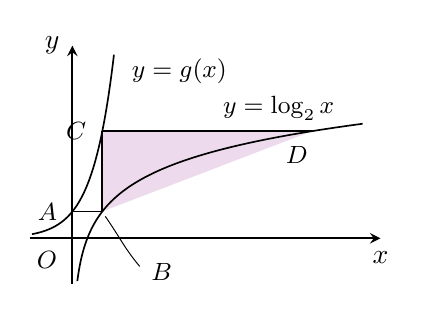
\begin{tikzpicture}[line width=0.6pt, x=0.19cm, y=0.34cm, >=stealth]
  \fill[violet!14] (2,1) -- (2,4) -- (16,4) -- cycle;
  \draw[->, line width=0.7pt] (-2.8,0) -- (20.6,0) node[below=1pt] {$x$};
  \draw[->, line width=0.7pt] (0,-1.7) -- (0,7.2) node[left=1pt] {$y$};
  \draw[domain=0.33:19.4, samples=200, smooth] plot (\x, {ln(\x)/ln(2)});
  \draw[domain=-2.7:2.78, samples=120, smooth] plot (\x, {pow(2,\x)});
  \draw (0,1) -- (2,1) (2,1) -- (2,4) (2,4) -- (16,4);
  \draw[line width=0.35pt] (4.5,-1.05) to[out=130,in=-55] (2.2,0.82);
  \node[font=\small, anchor=east] at (-0.35,1.0) {$\pt{A}$};
  \node[font=\small, anchor=west] at (4.6,-1.25) {$\pt{B}$};
  \node[font=\small, anchor=east] at (1.6,4.0) {$\pt{C}$};
  \node[font=\small, anchor=north] at (15.0,3.80) {$\pt{D}$};
  \node[font=\small, anchor=north east] at (-0.35,-0.12) {$\pt{O}$};
  \node[font=\small, anchor=west] at (3.3,6.25) {$y=g(x)$};
  \node[font=\small, anchor=west] at (9.4,4.85) {$y=\log_2 x$};
\end{tikzpicture}
